The task was created because the customers expressed concern for the reactiveness of the program, it sometimes felt slow and customers said it felt like nothing was happening.
It is important that responses from a mobile application happen somewhat quickly, as mentioned in~\cite{Roto:2005:NNF:1062745.1062747}, if an application takes more than 4 seconds to load or respond then other feedback than visual should be used.
Therefore it is decided that almost instantaneous feedback is important such that the users feel like the application is working quickly and effective.
This resulted in wanting a change of when calls were made in the PictoSearch application.

The current version of the PictoSearch application searches whenever the uses touches the search button on either the keyboard or on the GUI of the application.
The search button is located in the middle of the screen, to the left of the search field as can be seen on \myref{fig:screenshot_startup}.
\begin{figure}[h]
    \centering
    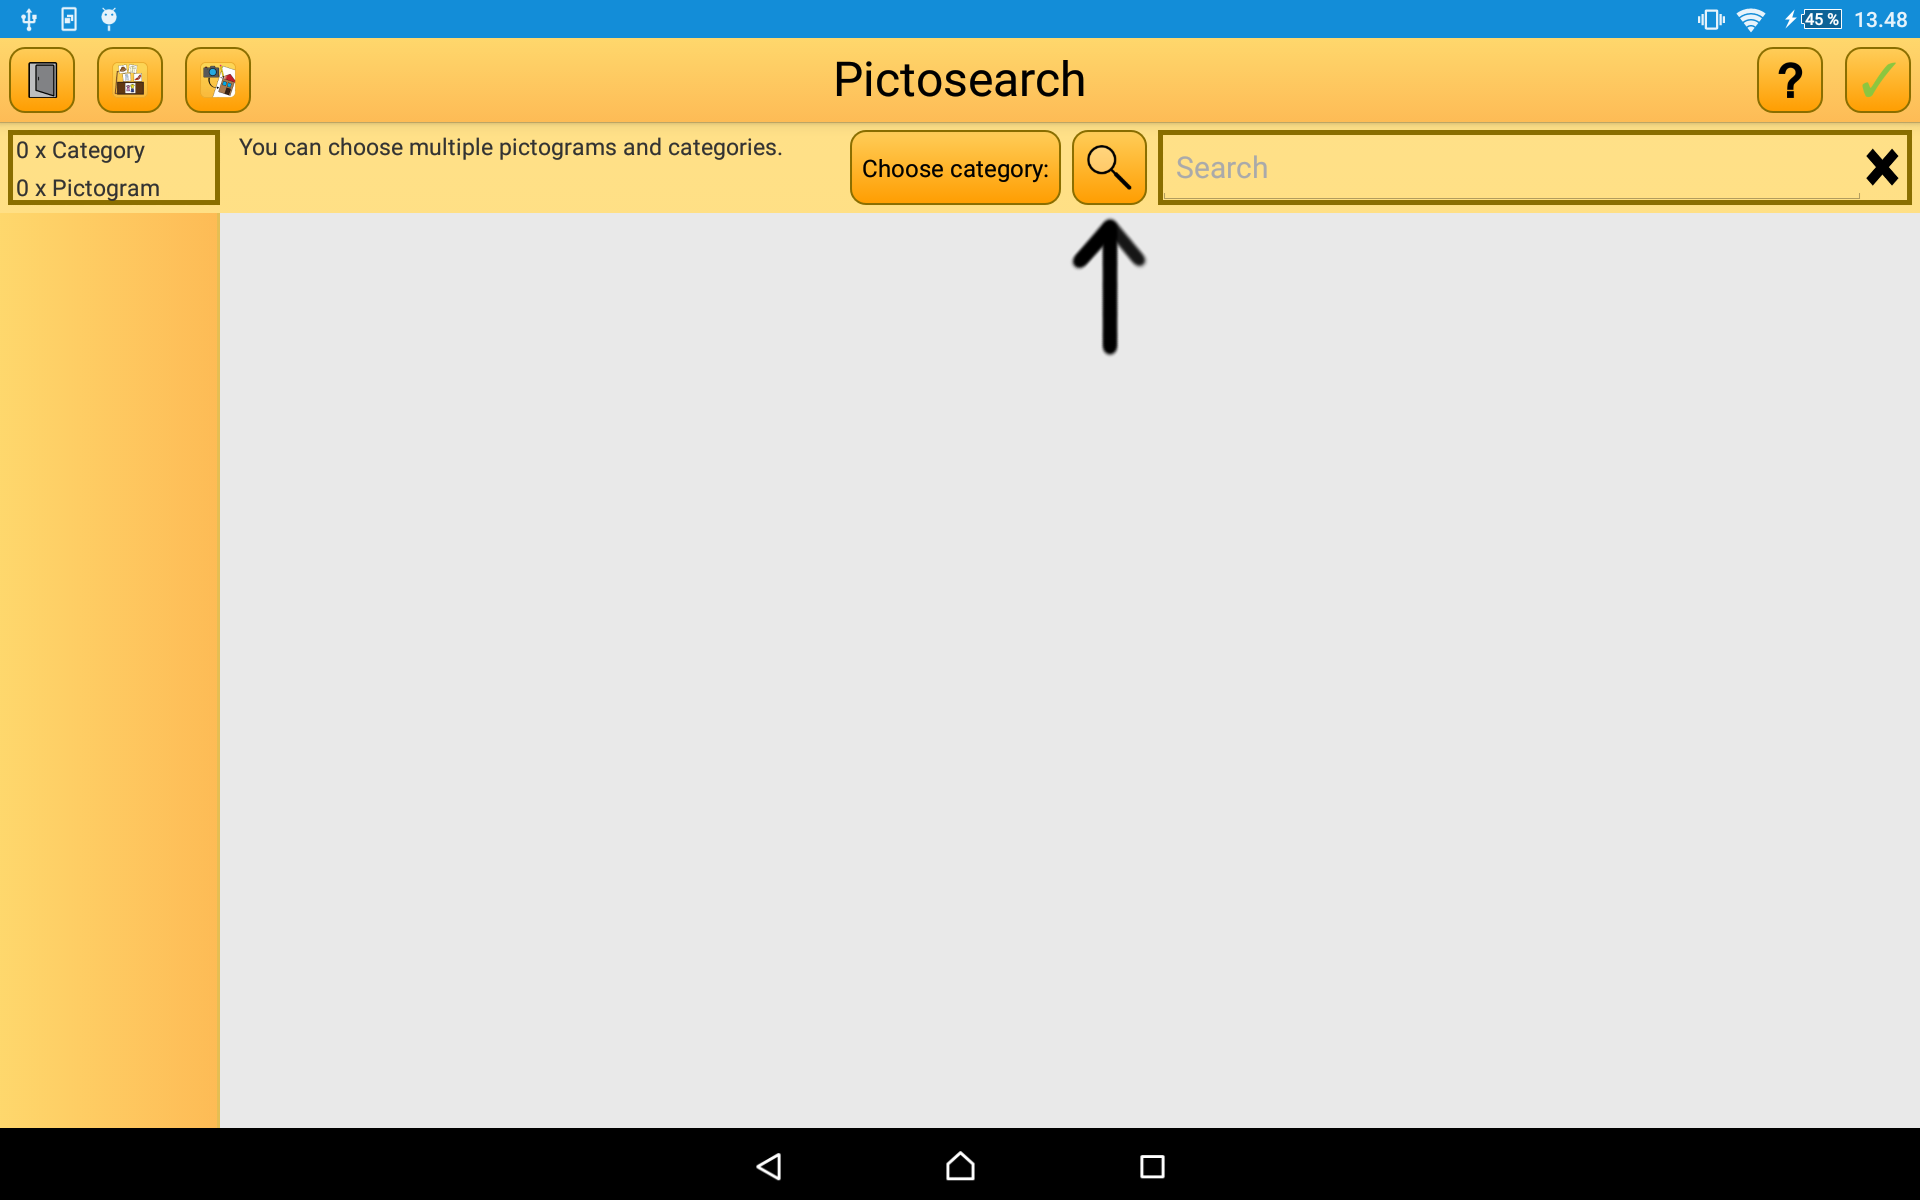
\includegraphics[width=0.8\textwidth]{figures/img/screenshots/old_startup.png}
    \caption{Screenshot of the initial view presented to the user when launching PictoSearch}\label{fig:screenshot_startup}
\end{figure}

\begin{figure}[h]
    \centering
    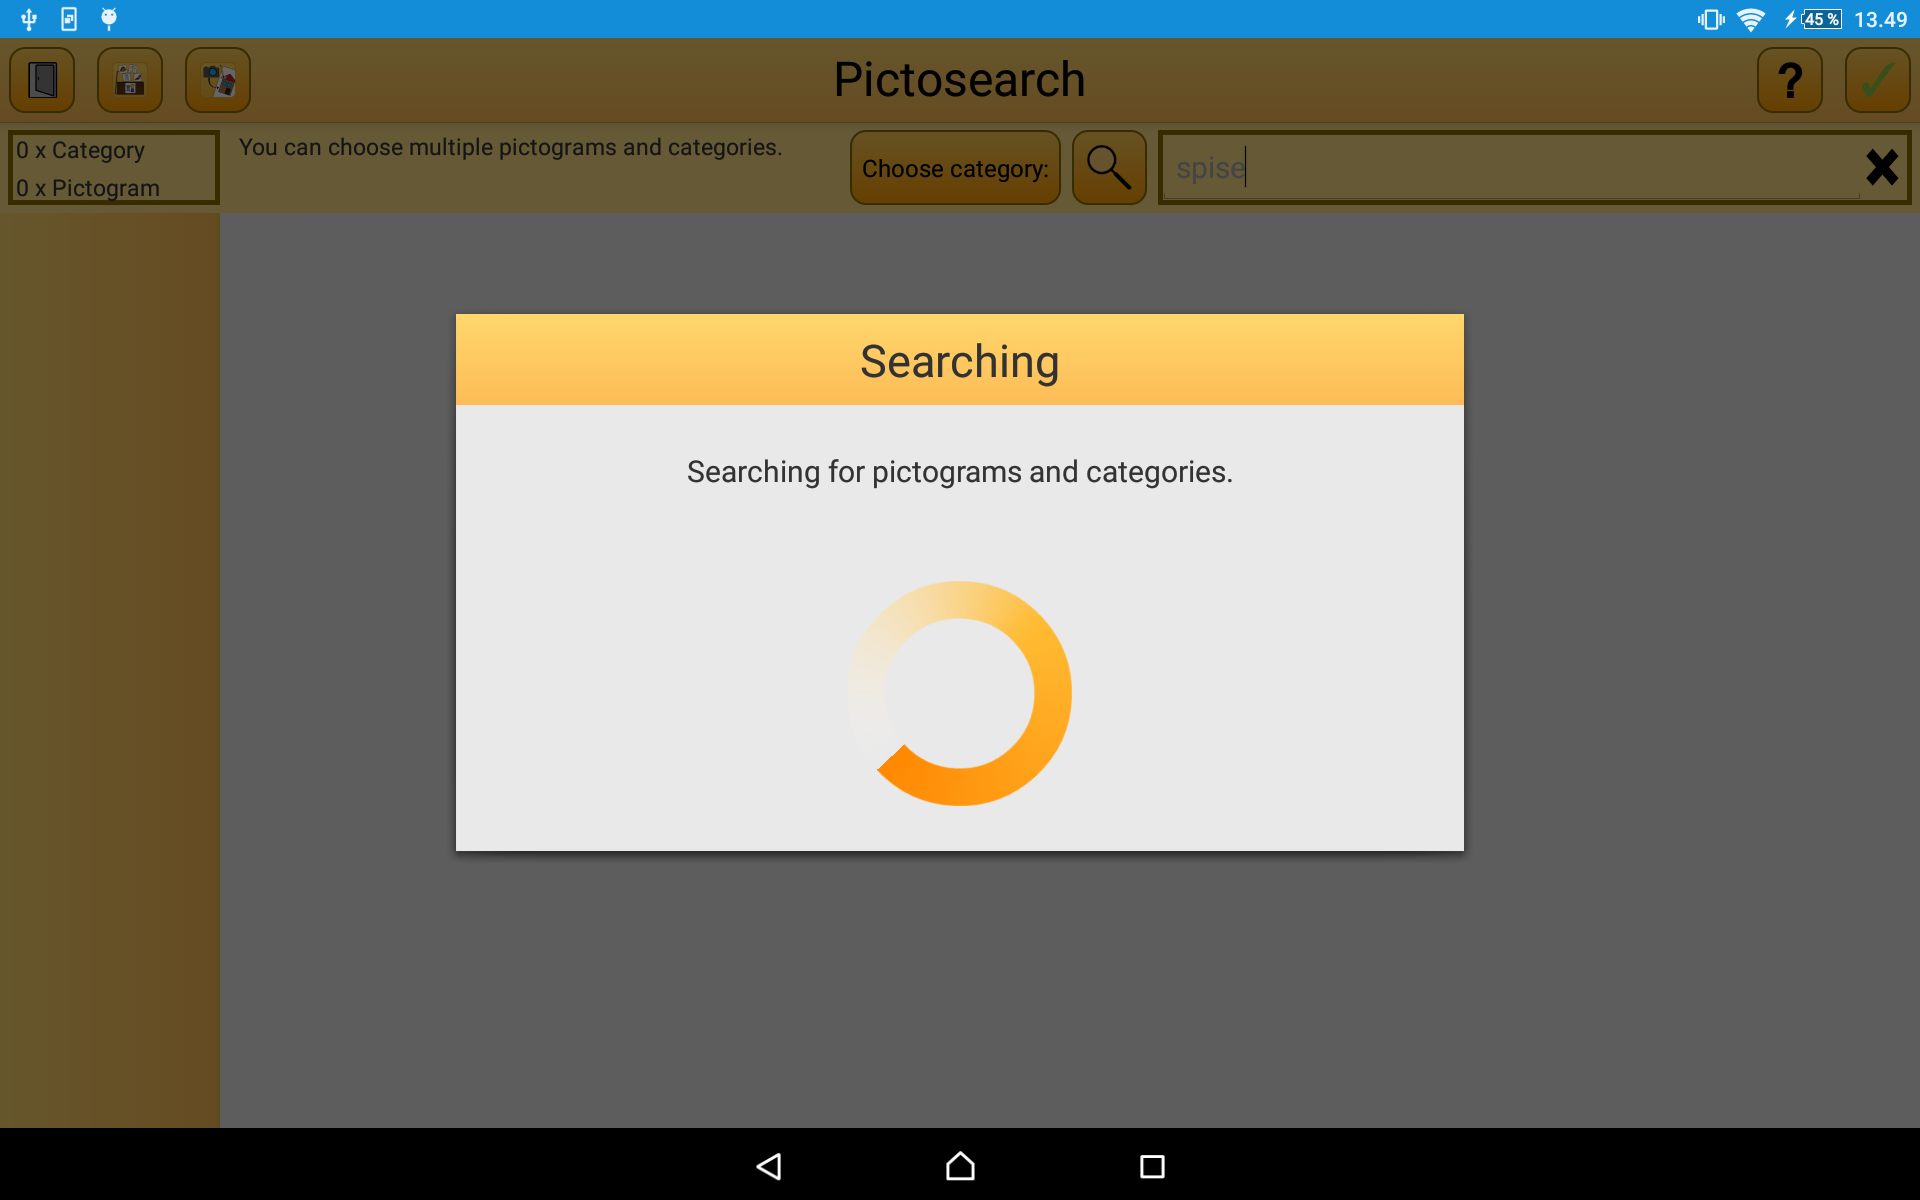
\includegraphics[width=0.8\textwidth]{figures/img/screenshots/old_dialog.png}
    \caption{Screenshot of the search spinner shown while searching in PictoSearch}\label{fig:screenshot_searchspinner}
\end{figure}
This has been changed such that a search happens whenever the text in the searchfield is changed.
Instead of the big slow search spinner which can be seen on \myref{fig:screenshot_searchspinner}, a new smaller text message is instead displayed which tells the user that the application is searching and what is is searching for. 
This search does not remove the software keyboard from the view, neither does it make you unable to type.
This is possible because the search is implemented as an async task, because of this any new search is queued behind the current search query.
This is fixed by calling \texttt{AsyncTask.cancel()}, which cancels the ongoing search call and makes it possible to start a new call immediately.
Because of this anytime a keystroke is made on the keyboard something should happen on the display other than simply filling out the searchfield, be it a text message explaining what is being searched for, or be it the resulting pcitograms returned from the search.
This means that there is instantaneous feedback for the user, which should give the feeling that the application is reacting to what the user is doing, and it does not feel like nothing is happening.

The search button can still be used, and will bring up the old search spinner as usually, but the button has been moved from the middle of the display to the right side of the display as can be seen on \myref{fig:screenshot_newstartup}.
This is a better fit as it resembles other common search engines such as google, and it is also the recommended way to display a search field according to the Niels Norman Group\footnote{https://www.nngroup.com/articles/magnifying-glass-icon/}.
It can also be seen on \myref{screenshot_newUI} that the cancel search button is only shown when there is actually something to remove from the search field, this removes the clutter of information otherwise produced from the old view.

\begin{figure}[h]
    \centering
    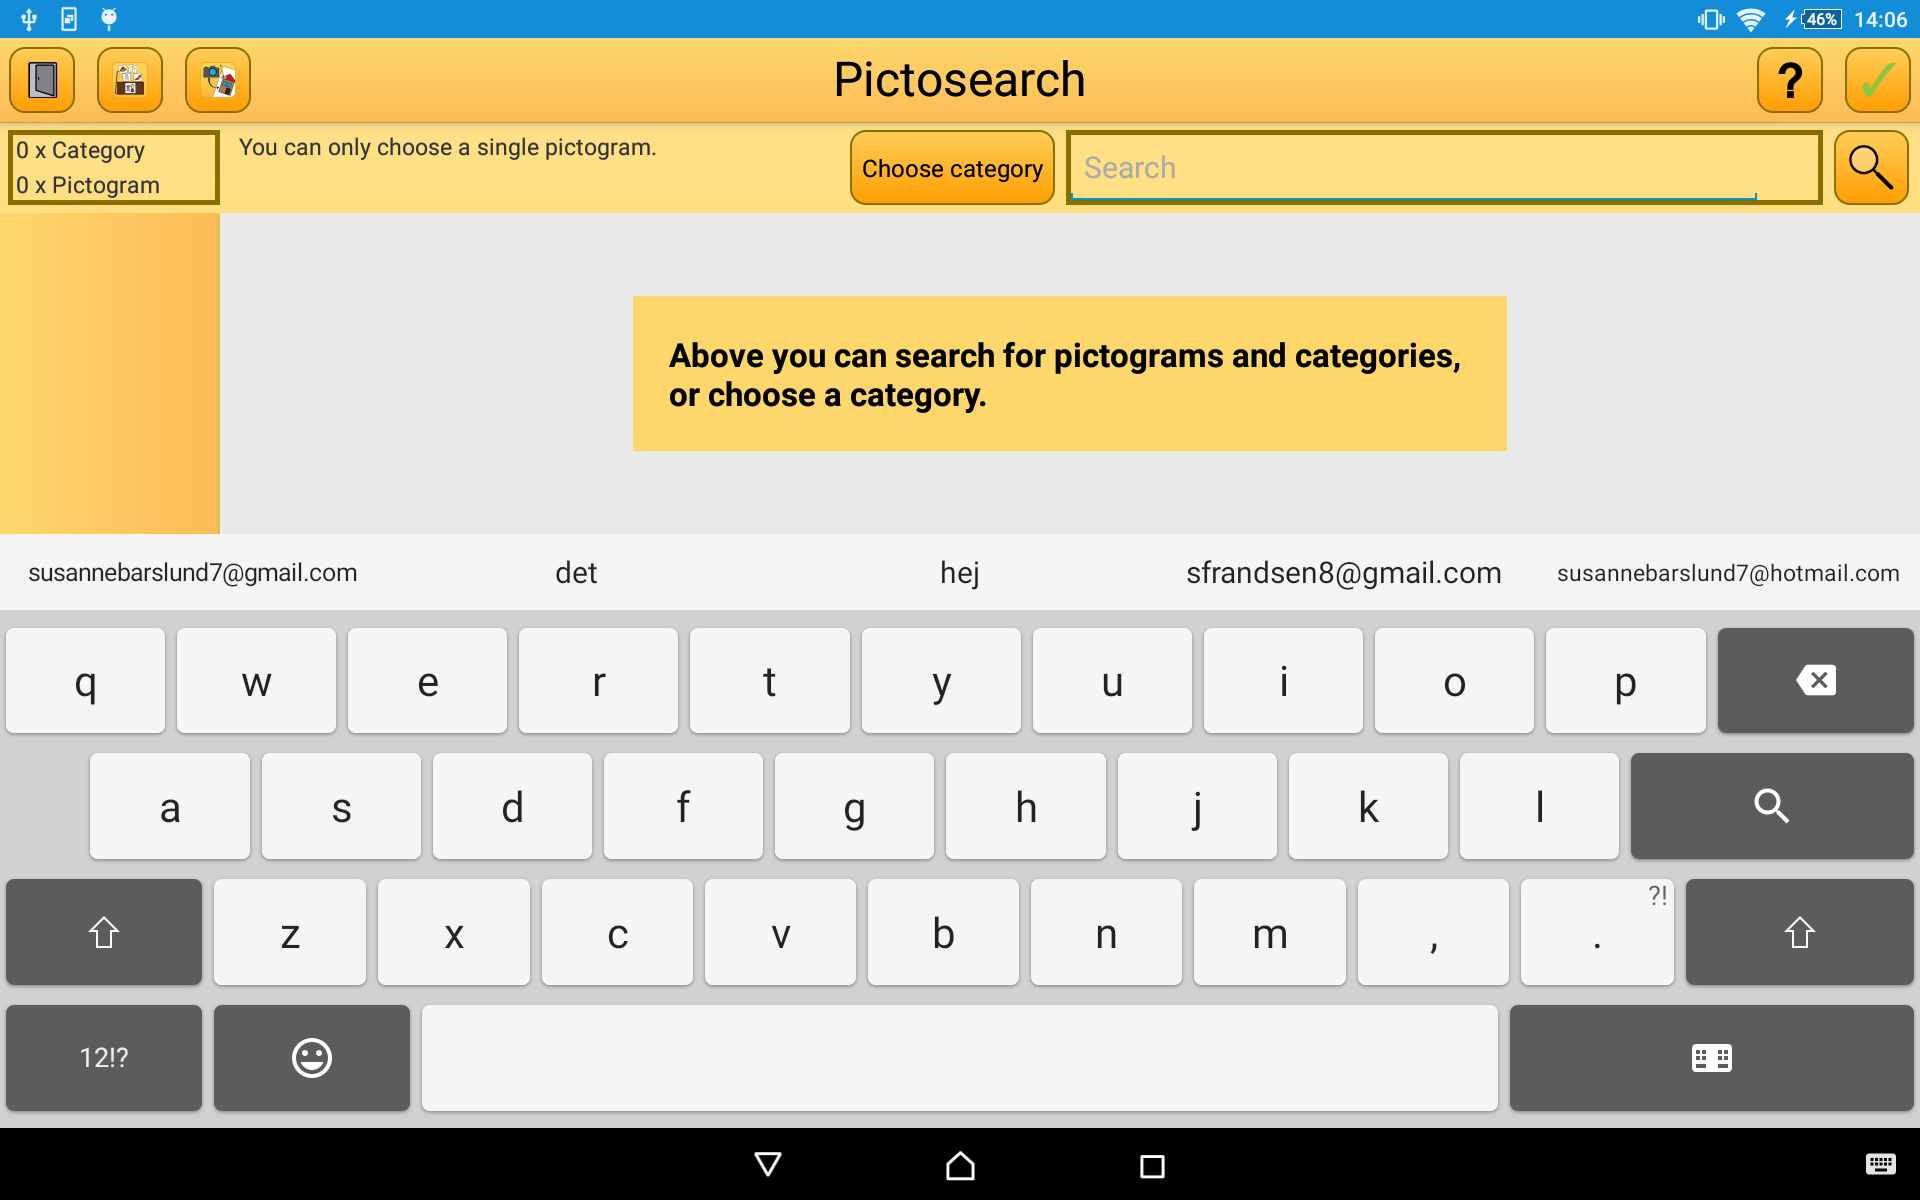
\includegraphics[width=0.8\textwidth]{figures/img/screenshots/new_startup.png}
    \caption{Screenshot of the new initial view in PictoSearch}\label{fig:screenshot_newstartup}
\end{figure}

\paragraph{Initial view}
Another change made to PictoSearch involves a task, which describes a need for modifications to be made to the initial view; This is the view that is presented to a user when launching PictoSearch.
In the current version, the user is presented with no useful information in the initial view as seen in \myref{fig:screenshot_startup}.
Initially this task involved showing somewhat random pictograms in the initial view, however we suspected that users might get confused by this, and believe that the pictograms shown were the only pictograms available in PictoSearch; therefore we simplified the task to assist the user in using PictoSearch.
As the aim of the workflow which involves PictoSearch is to search for pictograms, we set out to reduces the number of actions needed for such an operation. 
Furthermore we want to present some descriptive information to the user at any given time, such that it is clear what he or she should do to advance in the searching.
The first change is that the keyboard is forced to appear on the screen when launching PictoSearch, along with giving focus to the search field; this enables the user to start searching right away without having to press anything.
This new initial view, which also includes added informative text can be seen on \myref{fig:screenshot_newstartup}
